\setlength{\columnsep}{3pt}
\begin{flushleft}

\paragraph{What is loopback address?}
\begin{itemize}
	\item \textbf{127.0.0.1} is loopback IP address also called \textbf{localhost}.
	\item The \textbf{Class A}, 127.0.0.0 network address is reserved for loopback testing.
	\item Used to test whether NIC card is working properly or not.
	\begin{figure}[h!]
		\centering
		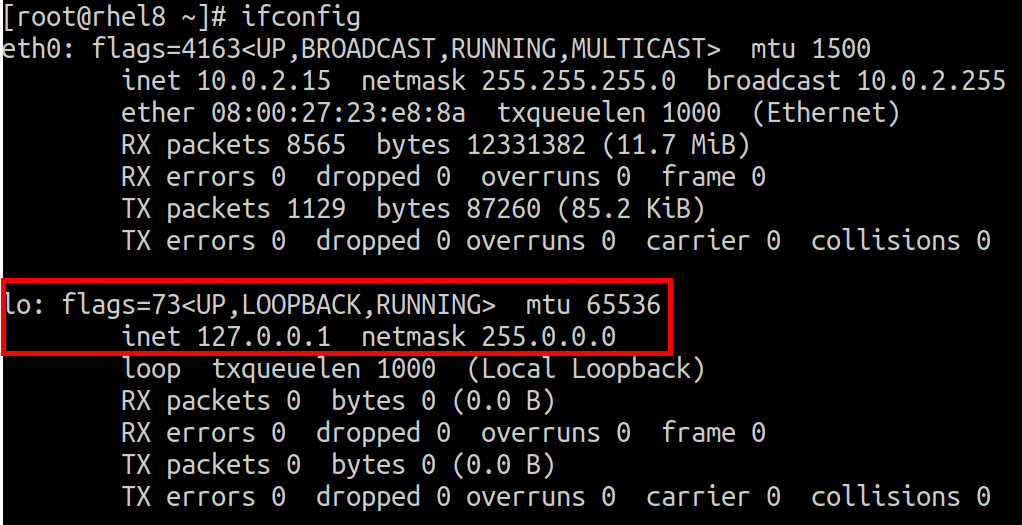
\includegraphics[scale=.28]{content/chapter14/images/loopback.png}
		\caption{Localhost IP}
		\label{fig:localhost_new}
	\end{figure}	

	\item You can ping localhost IP to check if your NIC card is working properly or not.
	\item Eg:
	\begin{figure}[h!]
		\centering
		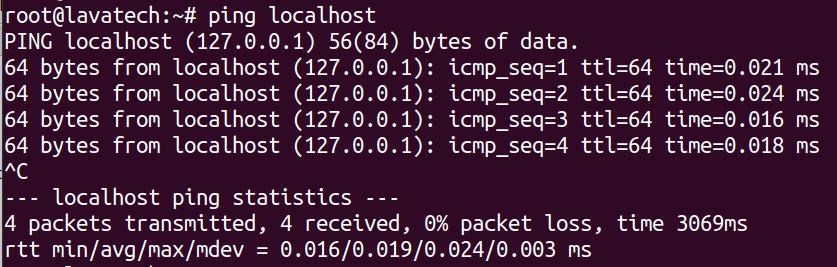
\includegraphics[scale=.35]{content/chapter14/images/ping.png}
		\caption{Localhost IP}
		\label{fig:localhost_new}
	\end{figure}	
\end{itemize}

\paragraph{What is 0.0.0.0 address?}

\begin{itemize}
	\item Can mean \textbf{"all IPv4 addresses on the system"}.
	\item Eg: If a system has two IP addresses, 192.168.1.1 and 10.1.2.1, and a server running on the system is configured to listen on 0.0.0.0, it will be reachable at both of those IP addresses.
\end{itemize}



\end{flushleft}
\newpage